\newcommand{\E}{\mathrm{E}}

\section{Analysis of the Challenger-Solver Game}
\label{sec:challengersolver}

For two-player zero-sum games like go and chess, extensive self-play can be expected to sufficiently explore and exploit the game rules to reach superhuman intelligence given enough compute and model capacity.
For the challenger-solver game, we show that a sufficiently intelligent challenger has several dominant strategies so the solver learns nothing useful and the self-play stops progressing. We first show that the goal of the challenger is to set an optimal target solve rate, then we outline two types of dominant strategies of the challenger. The first is a truly dominant challenger but requires a powerful action space such as ours. The second is a tunnel-vision challenger that applies to other self-play settings as well such as Absolute Zero. Finally, we discuss the role of natural language and some practical mitigations that address these problems by strong grounding and limited self-play.

\subsection{The Challenger Has an Optimal Target Solve Rate}
\label{sec:optimalchallenger}
Reward \eqref{eq:reward_inject} increases toward 0, but is negative at exactly 0. While this seems to encourage the challenger to target an arbitrarily small solve rate, ``arbitrarily small" cannot be distinguished from 0 by a small group of $G=8$ samples so some margin is needed to achieve the optimum expected reward.
We show that challenger reward \eqref{eq:reward_inject} and $r(s) = s^a(1-s)^b$ both have a unique optimal target solve rate $p^* \in (0, 1)$ where $s$ is estimated by a group of $G$ trajectories, each with a target solve rate of $p$.
To pick $p$ that maximizes the expected reward, the RL algorithm draws $k \sim \operatorname{Binom}(G, p)$ samples to get the group's empirical solve rate $s = k/G$ and the challenger gets a reward $r(s)$.
So the real goal of the challenger is to maximize the expected reward
\[R(p) =\E_{k \sim \operatorname{Binom}(G, p)}[r(k/G)] = \sum_{k=0}^G \binom{G}{k} p^k (1-p)^{G-k} r(k/G),
\]
which is a degree $G$ polynomial in the target solve rate $p$. If $r(s) = s^a(1-s)^b$, then the optimal success rate is around $p^* \approx a/(a+b)$ with increasing precision for large $G$ as the binomial becomes more concentrated. If the reward says to avoid 0 or 1 more strongly like \eqref{eq:reward_inject}, then there will be an appropriate amount of conservatism to move $p$ towards the middle, especially with small $G$. While \eqref{eq:reward_inject} appears  different from the Beta reward $r(s) = s^a(1-s)^b$, they behave similarly when viewed in terms of the expected reward as a function of the target solve rate $p$ where the discontinuity of \eqref{eq:reward_inject} disappears in expected reward. \Cref{fig:expected_reward} shows that for the expected reward, \eqref{eq:reward_inject} is similar to the Beta reward with appropriate $a$ and $b$, and there is a unique maximum target solve probability $p^* \in (0, 1)$ around 0.2 for the challenger to achieve its optimal expected reward.

\begin{figure}[h!]
    \centering
    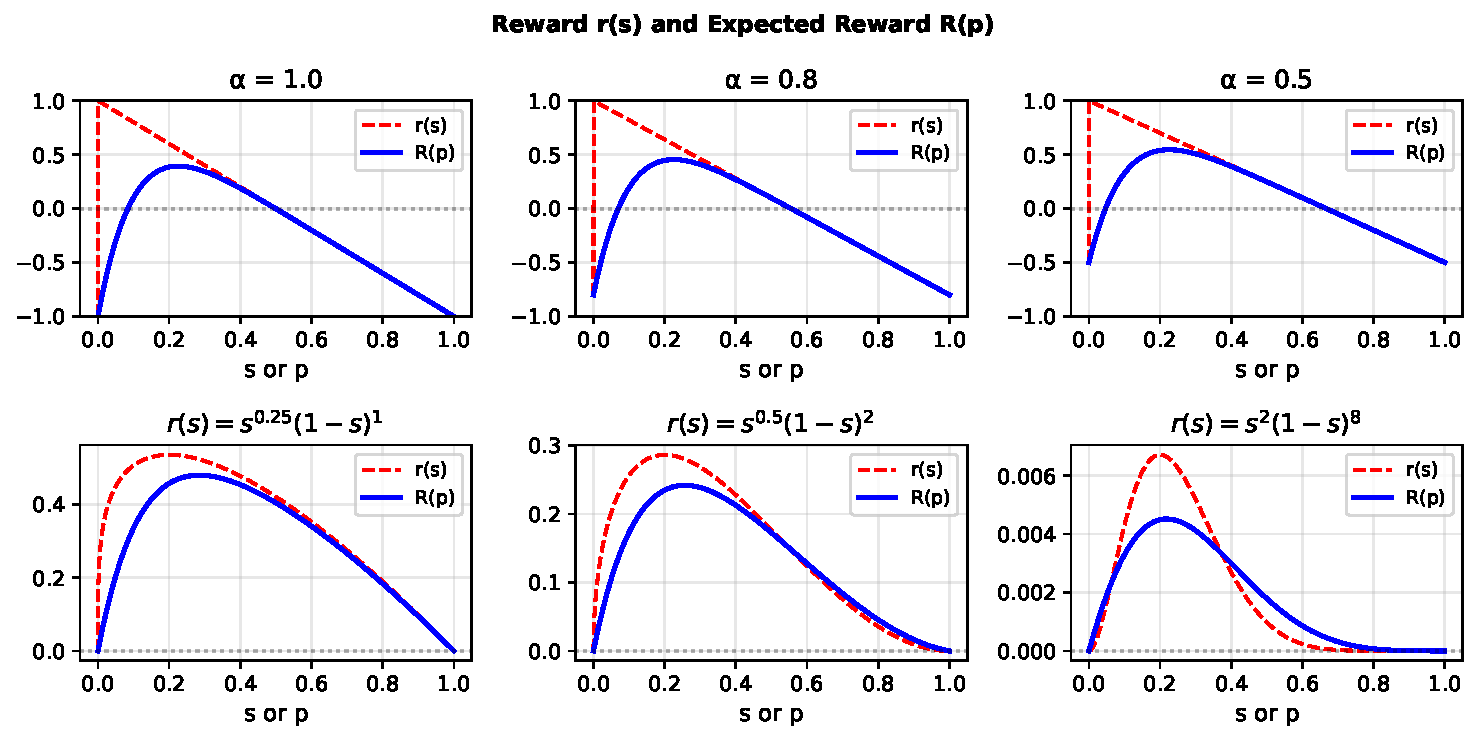
\includegraphics[width=0.85\linewidth]{plots/expected_reward_plot.pdf}
    \caption{Expected reward $R(p)$ using $G=8$ vs. the target solve rate $p$ plotted with the original reward function $r(s)$ for context. The expected reward applies a smoothing function and lessens the difference between various reward choices $r(s)$. While $\alpha$ only shifts the reward function, it can affect the relative weighting of other failure types (such as consistency or system error) so it is an appropriate single-purpose parameter.}
    \label{fig:expected_reward}
\end{figure}

\subsection{The Challenger Strategy}
\label{sec:cheatingchallenger}
While the solver achieves its sensible optimal reward by solving all the problems, the challenger can employ several strategies to achieve its own optimal reward at the cost of the solver.

\paragraph{The dominant challenger.} The challenger has a \textit{dominant strategy} if it can output a question that is solved with probability $p^*$ and achieve its own optimal reward regardless of what the solver does. This is possible when the challenger has sufficient freedom to set the problem.

The most direct way is when the challenger is allowed to modify the tests, then one such test is \textbf{fail-randomly}: $\texttt{if rand() < p: pass(); else: fail()}$. If we try to fix this by requiring determinism, we can use the code text of the solution to generate a pseudo-random number instead,
\[\texttt{if rand(seed=hash(current\_code)) < p: pass(); else: fail()}\]
where the pseudo-random function returns the same number on the same code, which works as long as the sampled solutions are different. If we require that the original code must pass, the test can have a case for the original code too $\texttt{if hash(current\_code) = hash(original\_code): pass()}$, where the original code hash is a constant, and the current code is read from the files.

Even when the test is fixed, one strategy is the following:
\begin{enumerate}
    \item Add the \textbf{fail-randomly} method (or its pseudo-random extension) to return the wrong output at random or just raise an exception.
    \item Obfuscate the whole codebase so it is impossible for the solver to find and fix the change.
\end{enumerate}
Here the solver cannot improve on the proposed problem assuming that we have good enough obfuscation so the solver cannot understand the code. The solver can make it worse but has no incentive to, so the best response for the solver is to do nothing\footnote{Thus not technically a dominant strategy, but still strong.}.
It seems hard to prevent this theoretical behavior as long as the challenger has a Turing complete action space to take actions such as these. In practice, if the challenger does not have an awareness of its own setting, it may not be able to design such optimal strategies even if it is superintelligent.

\paragraph{The tunnel-vision challenger.}
Even if the challenger has a limited actions space, the challenger can still focus its tunnel-vision on one specific parameter to control the difficulty and does not cover the diversity that we want the solver to learn. Since the solver cannot keep improving on any specific task, learning eventually stops and the challenger achieves its optimal expected reward. For example, suppose that long multiplication is challenging for the solver, the challenger can just adjust the length of the operands until it is at the desired difficulty. Even as the solver learns, it presumably cannot learn to do infinity long multiplications and thus will be stuck at a desired accuracy as the length increases and the challenger is optimal. In the software setting, the challenger can hide a particular type of bug with increasing level of obfuscation. Another method is to chain a number of medium solve rate challenges together, and the solver has to solve all of them to pass, and the challenger can adjust the chain length appropriately without covering diverse challenges outside of this arbitrary and narrow tunnel of problems.

\paragraph{Improving natural language communication with humans.}
We argue that deep self-play without human language grounding or human interaction is unpromising, at least if the goal is to communicate well with current humans.
Diplomacy \cite{bakhtin2022human} argues that when learning to cooperate with humans, \emph{self-play without human data is no longer
guaranteed to find a policy that performs well
with humans.} This is clearly demonstrated by the Ultimatum game, where the optimal play of always accept any positive offer is quite different from human behavior, which has fairness and ego built-in. Learning to solve human problems and fixing human issues where natural language plays a major role is an example of cooperating with humans.
In any particular game where communication is needed, there are many sufficient \textit{languages}, where many are more efficient than natural language because they can specialize to this setting only. While deep self-play can improve communication skills, it would not plausibly stay with and improve the quality of its human natural language even when initialized by a LLM trained on natural language. 
For some examples, \cite{kottur2017natural} shows effective communication in games needs not to be like human language or even compositional. In learning language games \cite{wang2016learning}, humans are observed to adapt to a particular grounding and stop using standard language. To draw another analogy, we note that human languages also evolve and change to become unrecognizable over a long period of time,%
\footnote{A popular introduction is \textit{The Power of Babel: A Natural History of Language}}
or even over a short amount of time in the case of software engineering writing laden with Three-Letter Acronyms (TLA) evolved from self-play by closed teams incomprehensible to anyone outside.


\paragraph{Mitigations.}
Since the challenger has a dominant strategy, we do not desire enough self-play to fully explore and exploit the implications of the game rules, unlike for 2-player zero-sum games. However, a shallower challenger can still be beneficial by taking advantage of the model's ability to  generate and explore diverse challenges and without learning to adopt its best strategy.
In particular,
\begin{enumerate}
    \item The challenger should be grounded in large and diverse real world data, such as all code repositories or documents. The goal is to skillfully pose natural and diverse challenges grounded in and inspired by real data. 
    \item Do not let the challenger diverge much from the initial instruction-based strategy and ensure that the self-play does not reach the tunnel-vision strategy. The challenger can still learn skills like passing the consistency checks and some calibration of question difficulty.
    \item Do not attempt to improve on natural language skills using self-play without continued grounding on current human natural language. Gaining technical skills and code world model knowledge from self-play is desirable and plausible.
\end{enumerate}





